\part{Phase Two: Implement Dashboard view with HTLM5/CSS3/JS + extend RESTfule
API}

\chapter*{Introduction}
\label{c_phasetwo}
On this section, we will experiment with different frameworks to improve the
tool in terms of UX and functionality. Also we will look for new ways to show
same data, just following a Lean approach and go step by step until the result
is the successful one.


\chapter{Facelift with Bootstrap}
There are few front end frameworks that help the web developer to build a
consistent, usable and responsive web, such as
Backbone\footnote{\url{http://backbonejs.or}}, 
Underscore\footnote{\url{http://underscorejs.org/}},
Skeleton\footnote{\url{http://www.getskeleton.com/}},
Foundation\footnote{\url{http://foundation.zurb.com/}},
Compass\footnote{\url{http://compass-style.org/}},
Bootstrap\footnote{\url{http://getbootstrap.com/}} and few others. With them
you cover the required features to build a web tool in a
single page and/or have responsive mobile web implementation using the latest
CSS3 and Saas extension, like Compass.

I started applying Bootstrap to the dashboard in a very straigt forward way and
getting awesome results a couple of hours later.

First thing to do is to import required libraries, such as main style sheet,
JavaScript extensions (that is required to get some fancy actions and effects)
and optional theme, as it is shown on the following code
\ref{f_facelift_bootstrap_code}, note that the library is loaded from the
closest server to the user as it is using \emph{MaxCDN.com} service
(\texttt{//maxcdn.bootstrapcdn.com/\ldots}), being a distributed replication
content system\footnote{Other similar system would be
\url{http://www.akamai.com}.}.

\begin{lstlisting}[style=html,breaklines=true,caption=Bootstrap\
required\ libraries,label=f_facelift_bootstrap_code]
<!-- Bootstrap http://getbootstrap.com/getting-started/ --> 
<!-- Latest compiled and minified CSS --> 
<link rel="stylesheet" href="//maxcdn.bootstrapcdn.com/bootstrap/3.2.0/css/bootstrap.min.css">

<!-- Optional theme -->
<link rel="stylesheet" href="//maxcdn.bootstrapcdn.com/bootstrap/3.2.0/css/bootstrap-theme.min.css">

<!-- Latest compiled and minified JavaScript -->
<script src="//maxcdn.bootstrapcdn.com/bootstrap/3.2.0/js/bootstrap.min.js"></script>
<!-- Bootstrap -->
\end{lstlisting} 

Once we have the style sheet loaded, we just need to apply to our html entities
the proper class and role and result is just so fancy as you can see on the
following \reffigure{f_facelift_bootstrap},
\reffigure{f_facelift_bootstrap_2} and \reffigure{f_facelift_bootstrap_3}.

\begin{figure}[ht!]
	\centering
   	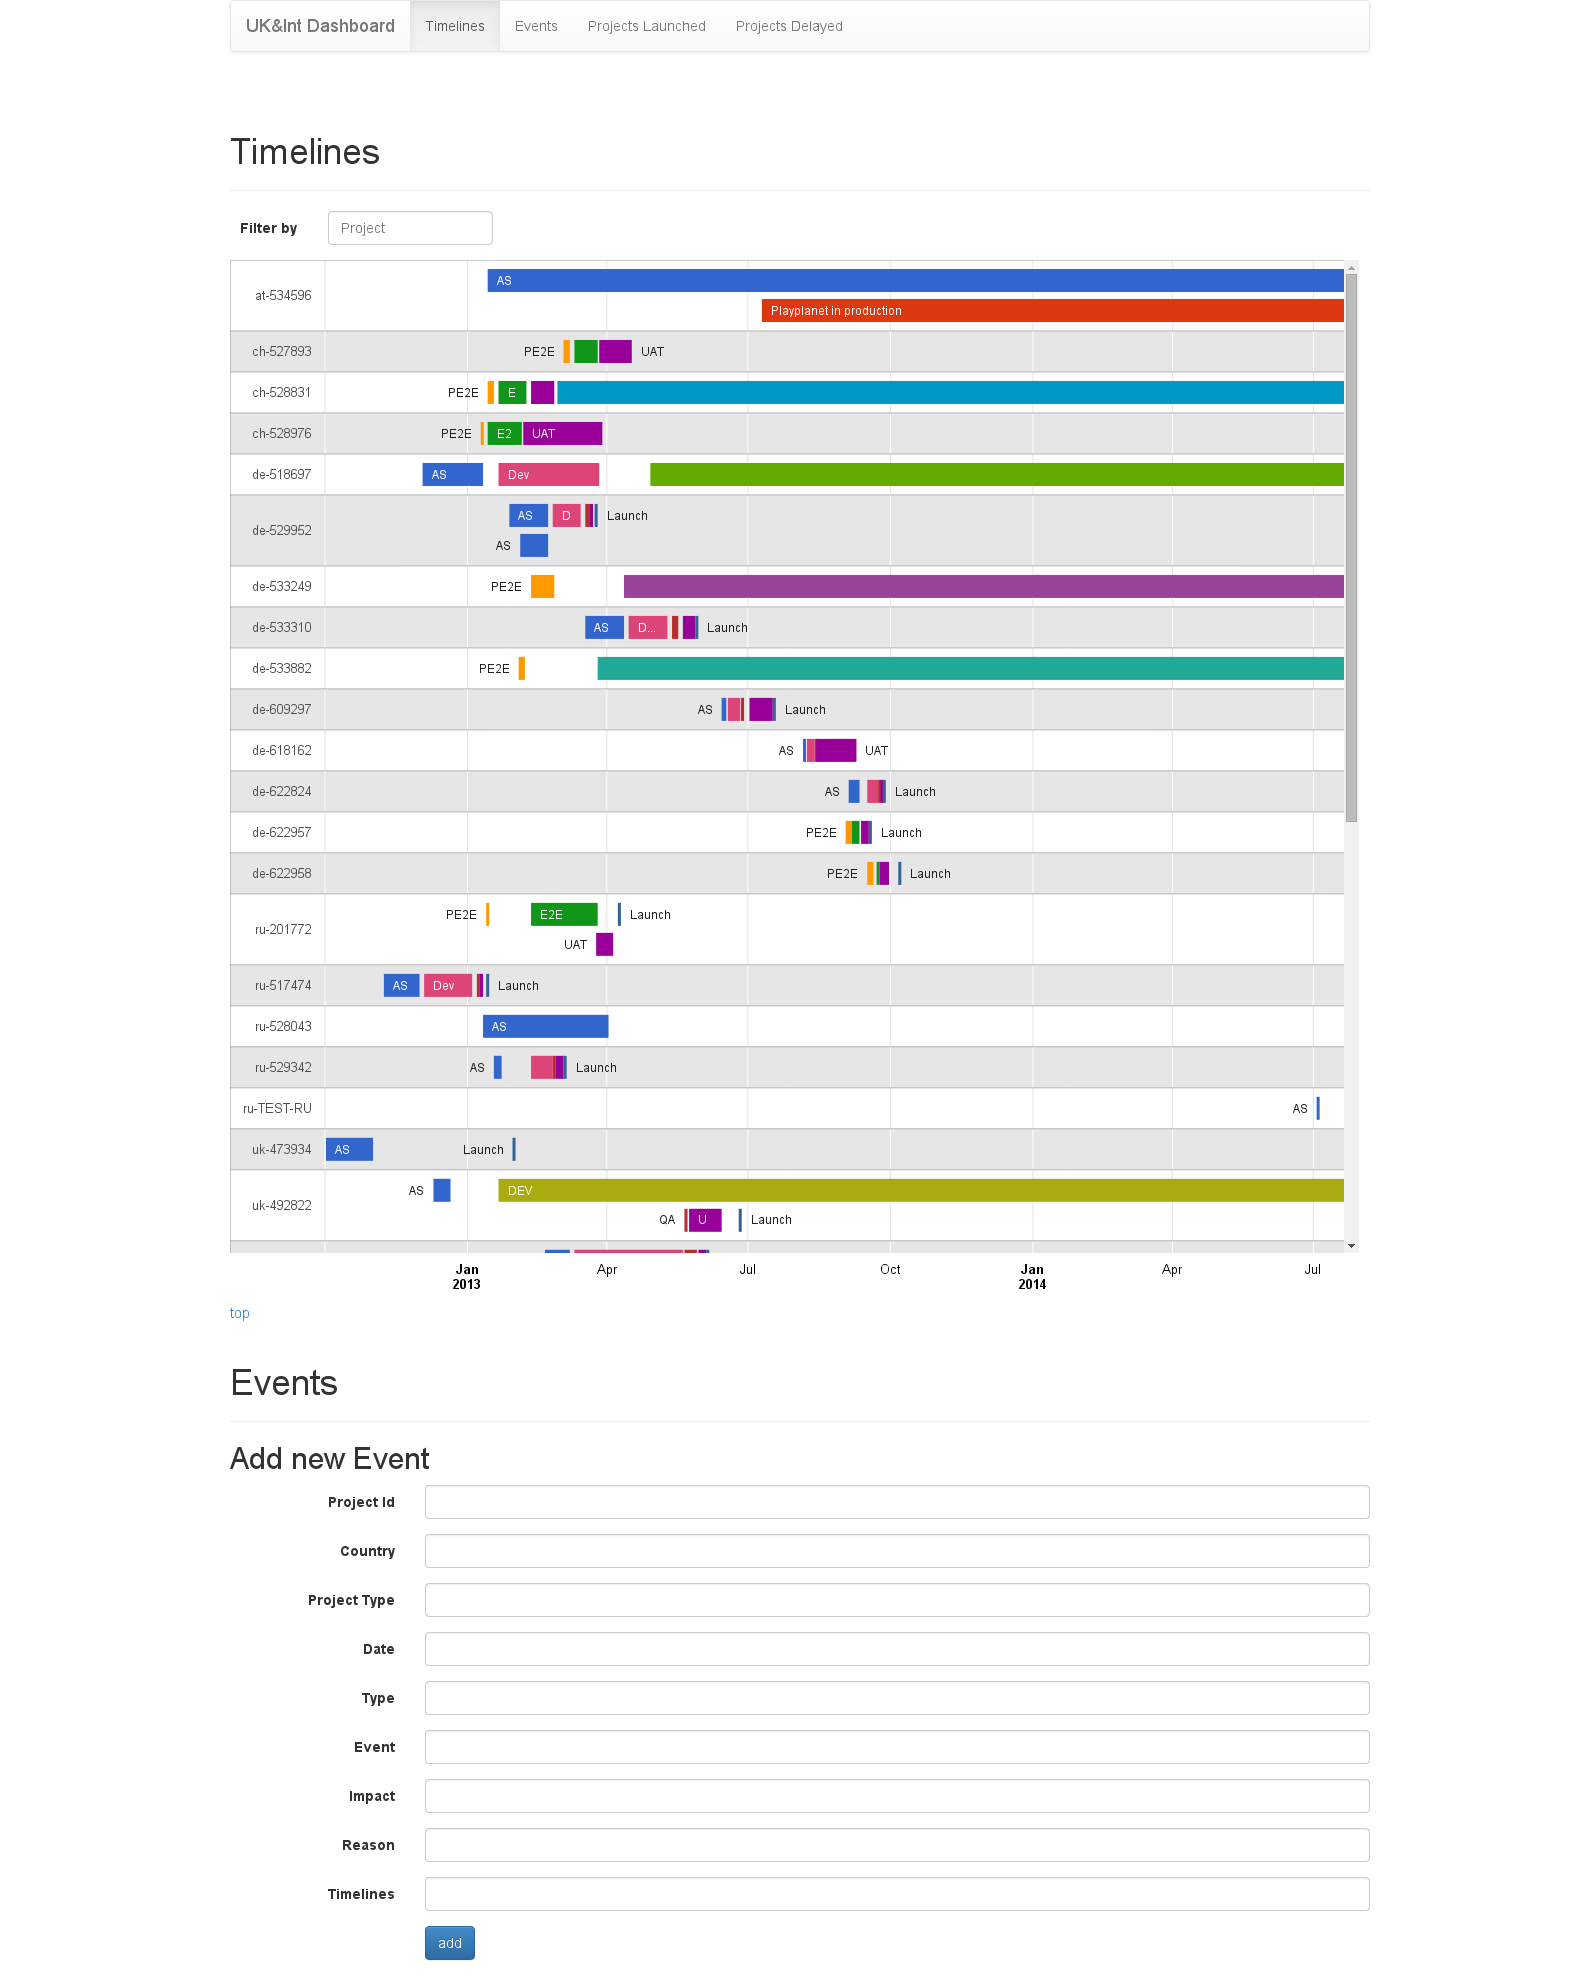
\includegraphics[width=1\textwidth]{./resources/dashboard_after_bootstrap_1.png}
   	\caption{Dasboard look and feel after apply Bootstrap style sheet (1)}
   	\label{f_facelift_bootstrap}
\end{figure}

\begin{figure}[ht!]
	\centering
   	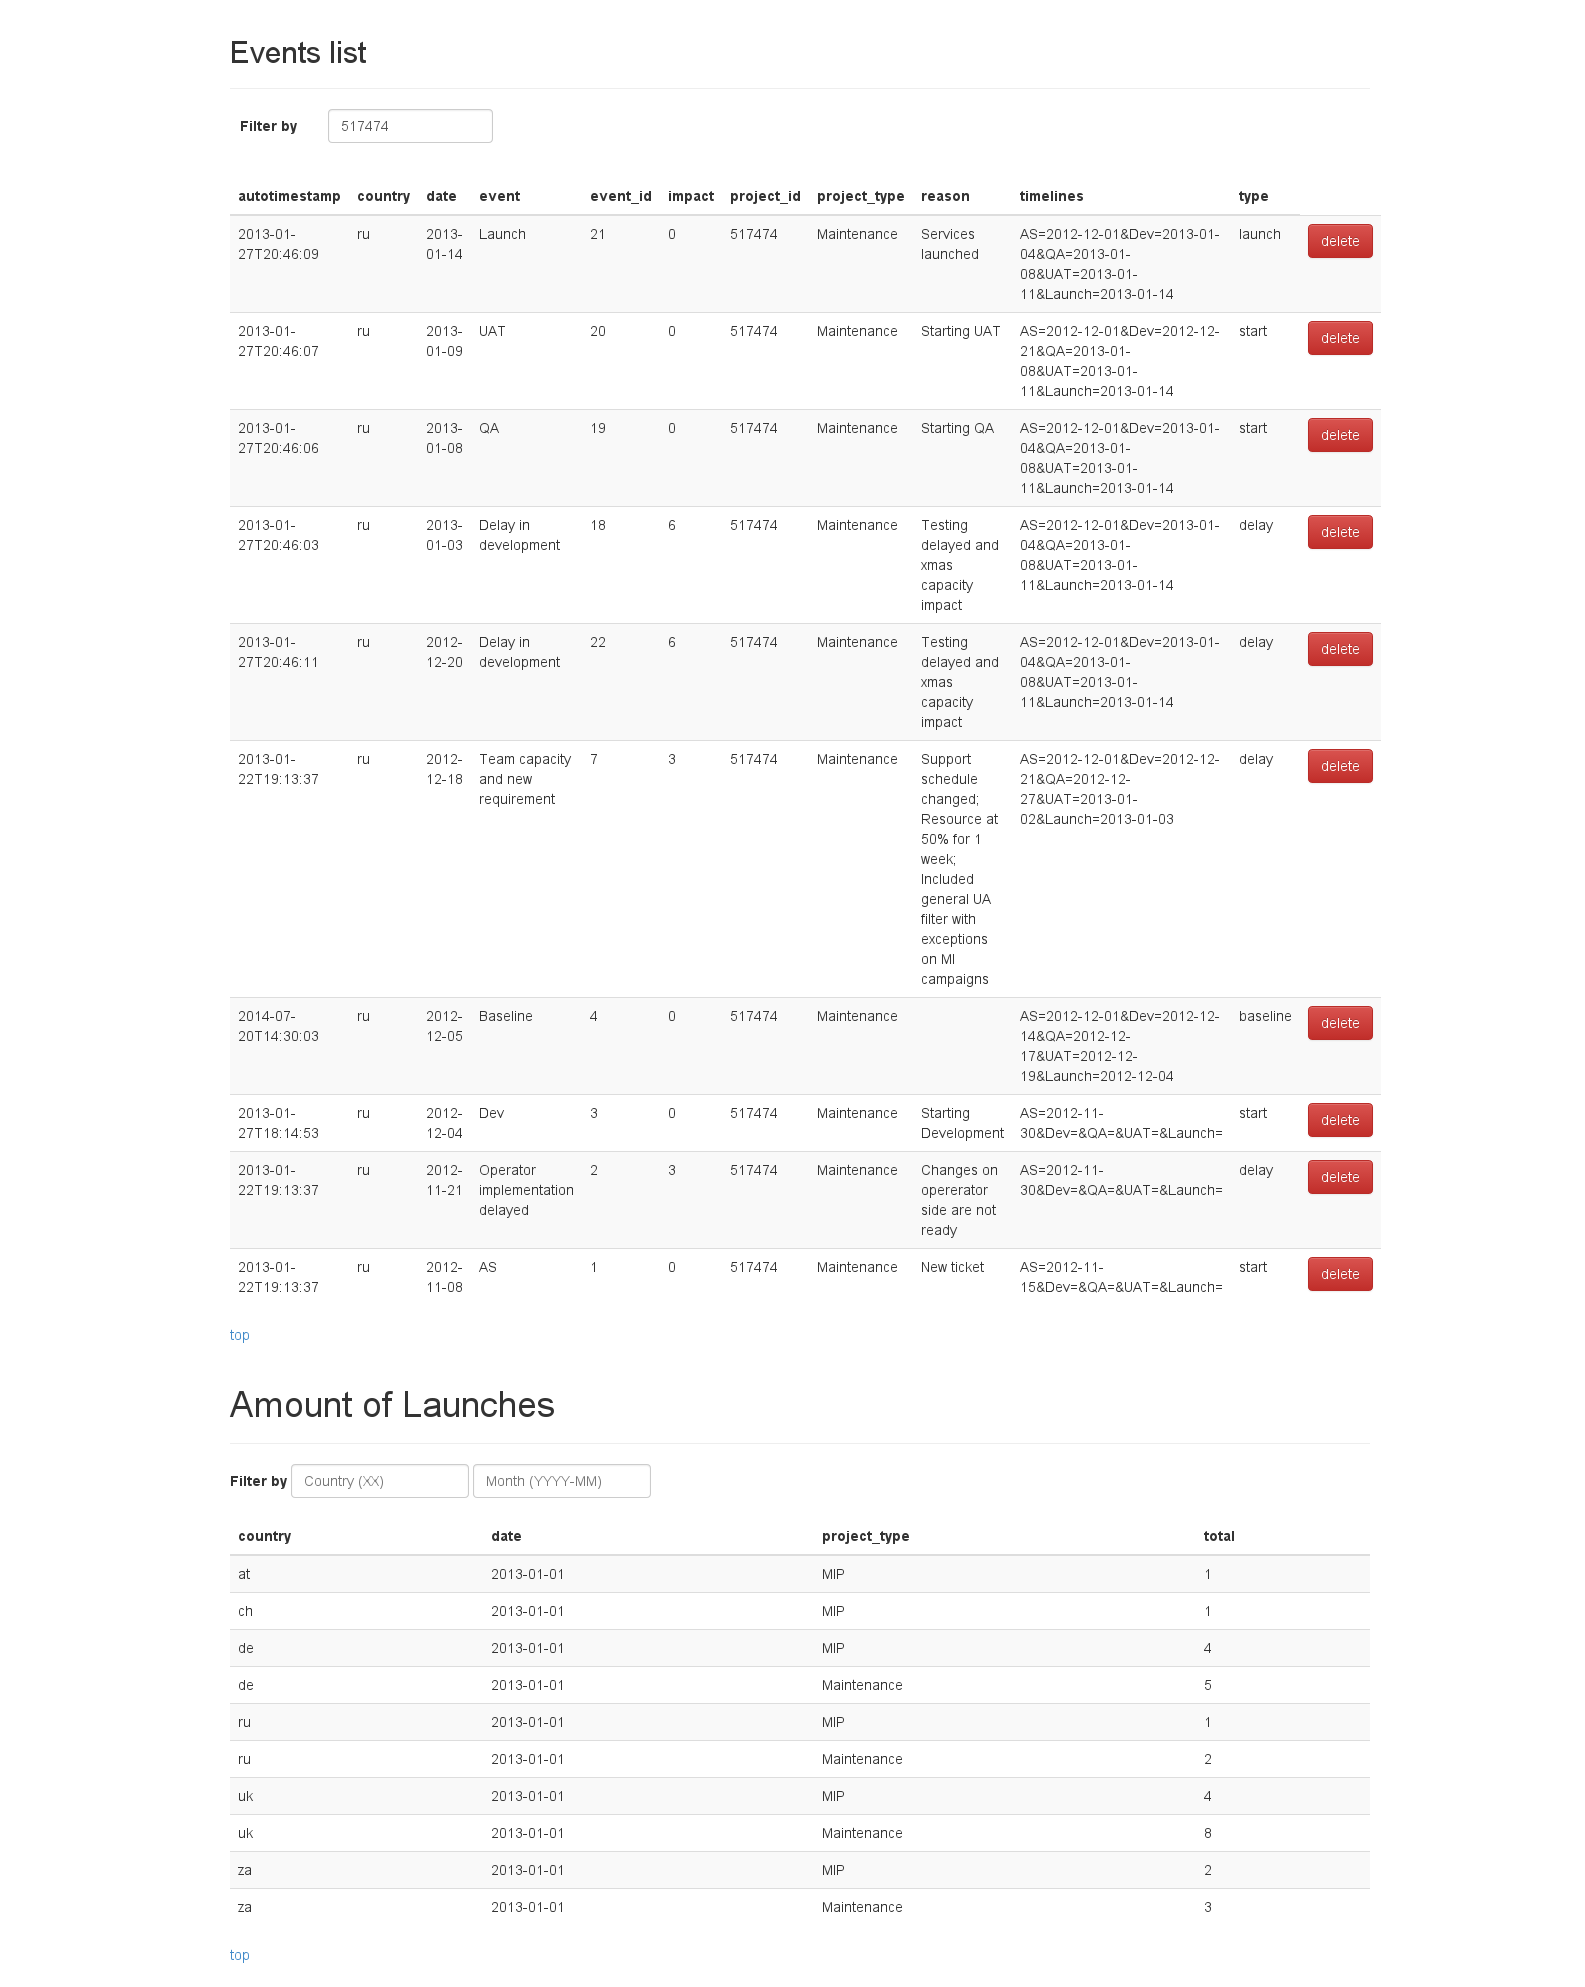
\includegraphics[width=1\textwidth]{./resources/dashboard_after_bootstrap_2.png}
   	\caption{Dasboard look and feel after apply Bootstrap style sheet (2)}
   	\label{f_facelift_bootstrap_2}
\end{figure}

\begin{figure}[ht!]
	\centering
   	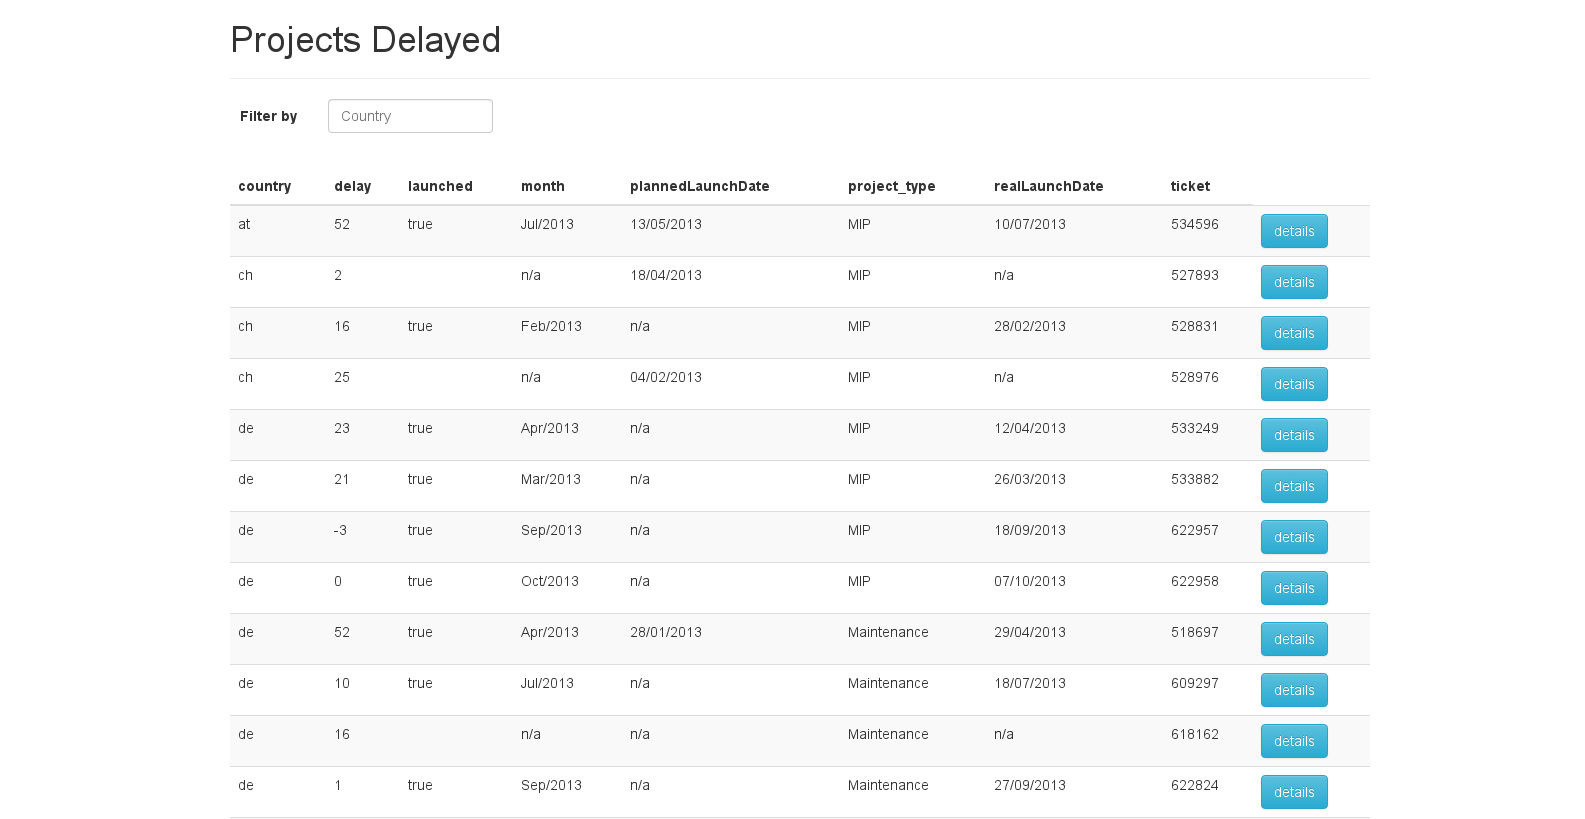
\includegraphics[width=1\textwidth]{./resources/dashboard_after_bootstrap_3.png}
   	\caption{Dasboard look and feel after apply Bootstrap style sheet (3)}
   	\label{f_facelift_bootstrap_3}
\end{figure}

\chapter{Extending Dashboard with Elasticsearch and Kibana}
Working on this currently and see if is feasible to implement the searching and
data calculation required for the reports based on Elasticsearch. The
main interesting point here is that we can change the way that we have been
thinking about the data on this project, and switch it from a relational data
model (MySQL), to a noSQL approach using Document model (JSON), something that our
application already uses :)

Don't know where it will end, but let's see and have fun with it along the
process.

